%%%%%%%%%%%%%%%%%%%%%%%%%%%%%%%%%%%%%%%%%
% Short Sectioned Assignment
% LaTeX Template
% Version 1.0 (5/5/12)
%
% This template has been downloaded from:
% http://www.LaTeXTemplates.com
%
% Original author:
% Frits Wenneker (http://www.howtotex.com)
%
% License:
% CC BY-NC-SA 3.0 (http://creativecommons.org/licenses/by-nc-sa/3.0/)
%
%%%%%%%%%%%%%%%%%%%%%%%%%%%%%%%%%%%%%%%%%

%----------------------------------------------------------------------------------------
%	PACKAGES AND OTHER DOCUMENT CONFIGURATIONS
%----------------------------------------------------------------------------------------

\documentclass[paper=a4, fontsize=11pt]{scrartcl} % A4 paper and 11pt font size

\usepackage[T1]{fontenc} % Use 8-bit encoding that has 256 glyphs
\usepackage{fourier} % Use the Adobe Utopia font for the document - comment this line to return to the LaTeX default
\usepackage[english]{babel} % English language/hyphenation
\usepackage{amsmath,amsfonts,amsthm} % Math packages
\usepackage{amssymb}
\usepackage{kotex}
\usepackage{lipsum} % Used for inserting dummy 'Lorem ipsum' text into the template
\usepackage{graphicx}
\usepackage[normalem]{ulem}
\usepackage{mdframed}
\usepackage{sectsty} % Allows customizing section commands
\allsectionsfont{\centering \normalfont\scshape} % Make all sections centered, the default font and small caps
\usepackage{tensor}
\usepackage{setspace}
\usepackage{twoopt}
\usepackage{fancyhdr} % Custom headers and footers
\pagestyle{fancyplain} % Makes all pages in the document conform to the custom headers and footers
\fancyhead{} % No page header - if you want one, create it in the same way as the footers below
\fancyfoot[L]{} % Empty left footer
\fancyfoot[C]{} % Empty center footer
\fancyfoot[R]{\thepage} % Page numbering for right footer
\renewcommand{\headrulewidth}{0pt} % Remove header underlines
\renewcommand{\footrulewidth}{0pt} % Remove footer underlines
\setlength{\headheight}{13.6pt} % Customize the height of the header

\numberwithin{equation}{section} % Number equations within sections (i.e. 1.1, 1.2, 2.1, 2.2 instead of 1, 2, 3, 4)
\numberwithin{figure}{section} % Number figures within sections (i.e. 1.1, 1.2, 2.1, 2.2 instead of 1, 2, 3, 4)
\numberwithin{table}{section} % Number tables within sections (i.e. 1.1, 1.2, 2.1, 2.2 instead of 1, 2, 3, 4)

\setlength\parindent{0pt} % Removes all indentation from paragraphs - comment this line for an assignment with lots of text

%----------------------------------------------------------------------------------------
%	DEFINITION & THEOREM
%----------------------------------------------------------------------------------------

\theoremstyle{plain}
\newtheorem{thm}{Theorem} % reset theorem numbering for each chapter

\newmdtheoremenv{defn}{Definition} % definition numbers are dependent on theorem numbers
\newmdtheoremenv{exmp}{Example} % same for example numbers

%----------------------------------------------------------------------------------------
%	BLANCK COMMAND
%----------------------------------------------------------------------------------------

\newcommand{\Com}{,\Hs}
\newcommand{\Hs}{\hspace{0.1cm}}
\newcommand{\HS}{\hspace{0.5cm}}
\newcommand{\VS}{\vspace{0.3cm}}

%----------------------------------------------------------------------------------------
%	DIFFERENTIATE COMMAND
%----------------------------------------------------------------------------------------

\newcommand{\OD}[2]{\frac{d #1}{d #2}}
\newcommand{\PD}[2]{\frac{\partial #1}{\partial #2}}

%----------------------------------------------------------------------------------------
%	ETC COMMAND
%----------------------------------------------------------------------------------------

\newcommand{\BKS}[1]{\left( #1 \right)}

%----------------------------------------------------------------------------------------
%	TENSOR COMMAND
%----------------------------------------------------------------------------------------

\newcommandtwoopt{\KD}[2][\mu][\nu]{\delta^{#1}_{#2}}
\newcommandtwoopt{\CT}[2][\mu][\nu]{\tensor{A}{^#1 _#2}}
\newcommandtwoopt{\CTI}[2][\mu][\nu]{\tensor{\BKS{A^{-1}}}{^#1 _#2}}
\newcommand{\Tangent}{T_p (\Manifold)}
\newcommand{\Cotangent}{T^{*}_p (\Manifold)}
\newcommand{\Manifold}{\mathcal{M}}
\newcommand{\Basis}[1][\mu]{\BKS{\PD{}{x^{#1}}}_p}
\newcommand{\Basisnp}[1][\mu]{\BKS{\PD{}{x^{#1}}}}
\newcommandtwoopt{\Commutator}[2][X][Y]{\left[ #1 \Com #2 \right] }
\newcommandtwoopt{\RCommutator}[3][X][Y]{#1\BKS{#2(#3)} - #2\BKS{#1(#3)}}
\newcommandtwoopt{\ECommutator}[2][X][Y]{\BKS{#1^\nu \PD{#2^\mu}{x^\nu} - #2^\nu \PD{#1^\mu}{x^\nu}}}

%----------------------------------------------------------------------------------------
%	TITLE SECTION
%----------------------------------------------------------------------------------------

\newcommand{\horrule}[1]{\rule{\linewidth}{#1}} % Create horizontal rule command with 1 argument of height

\title{	
\normalfont \normalsize 
\textsc{Deparment of physics, Yonsei University} \\ [25pt] % Your university, school and/or department name(s)
\horrule{0.5pt} \\[0.4cm] % Thin top horizontal rule
\huge 바쁜 사람들을 위한 일반상대론 \\ % The assignment title
\horrule{2pt} \\[0.5cm] % Thick bottom horizontal rule
}

\author{Axect} % Your name

\date{\normalsize\today} % Today's date or a custom date

\begin{document}

\maketitle % Print the title

%----------------------------------------------------------------------------------------
%	PROBLEM 1
%----------------------------------------------------------------------------------------

\section{Introduction}

\onehalfspacing
\HS 아마도 이 글을 보게 되는 사람이 있다면 분명, 두 부류 중 하나이거나 혹은 두 부류 모두 일 것이다. 첫째는 그나마 정상적인 사람으로서 제목의 뒷부분을 보고 들어온 사람일 것이고 둘째는 좀 심각한 사람으로서 제목의 앞부분을 보고 들어온 사람이다.
그러나 필자는 아주 극도로 순수하므로 둘째의 부류는 전혀 모르니(?) 어쨌거나 본연의 취지에 맞게 일반상대론을 최대한 쉽게 설명하고자 한다. \footnotemark
\footnotetext{이에 대해선 구글에 검색만 해보아도 쉽게 정보를 얻을 수 있으므로 생략하겠다.}
너무나도 당연한 얘기겠지만, 일반상대론을 하려는데 특수상대론을 모르는 것은 어불성설이다. 그러나 이를 짚고 넘어가는 것은 바쁜 사람들을 위한 것이 아니게되니, 가급적이면 따로 공부를 해두길 바란다.\footnotemark
\footnotetext{필자는 Landau vol.2 - \emph{The Classical Theory of Fields}를 추천한다.}

\vspace{0.3cm}

\HS 그럼 본격적으로 시작하기전에 적어도 우리가 하려는 것이 무엇인지, 그리고 그것을 위해 무엇을 이용할 것인지에 대해 한번 따져보자. 먼저 우리가 하려는 것은 
수많은 두꺼운 일반상대론 서적들에게서 여러분들을 조금이나마 해방시켜주려는 것이다. 예를 들어 희대의 명저인 Wald 나 Hawking \& Ellis 같은 책들만 봐도 
매우 읽기 싫어지고 차라리 상대론을 포기하고 싶어지는 심정이 들 것이다. (아니라면 존경합니다.) 자, 그럼 여기서 아주 당연하게 물어볼 수 있다. 도대체 네가 뭔데 
저런 명저들에게서 해방을 시켜주겠다는 거냐? 당연히 본인은 그럴만한 능력을 지니지 않았고 또한 그 책들에 있는 내용을 모두 다룰 생각도 전혀 없다. 다만, 적어도 
조금 쉬운 길을 알고 있고 그 길을 걷는 것만으로도 꽤나 득이 될 것이기에 이 짓을 하는 것이다. (사실은 자기만족겸 내용복습겸 정리라는 건 안 비밀.)  그럼 다음으로 어떻게? 가 관건이 될텐데 본인은 상대론 공부를 Landau, Hobson
 등과 같은 좀 더 Physical phenomena 위주의 책들 부터 Harvey Reall의 엄청난 강의 자료 까지 총 3-4개의 자료로 공부를 해보았으므로 대충대충 짜집기 하여서 
 진행하면 그래도 조금은 볼만 할 것이다. 물론 그 중에서도 엄지 손가락은 있기 마련인데, 여기서는 Harvey Reall이 주로 이용될 것이다.\footnotemark
 \footnotetext{사실 이것 자체가 엄청난 상대론 요약판!}
 따라서 이 강의보다 좀 더 엄밀함을 원한다면 Harvey Reall을 보시고, 거기에서 더 많은 내용들을 원한다면 Wald를 보는 것을 권한다. 자, 그럼 이제 본론으로 돌아가보자.
 
 \vspace{0.3cm}
 
 \emph{상대론이란 무엇인가?}
 
 \vspace{0.3cm}
 
 간단하게 설명하자면 시간과 공간을 하나로 엮은 것이자 그 유명한 $E=mc^2$ 을 포함하고 있는 이론이다. 이론의 특성상 상대론도 몇몇 가정들로부터 유도 되었는데, 특수상대론은 빛의 속도가 유한함에서, 일반상대론은 중력과 관성력이 구분불가능하다는 등가원리(Equivalence principle)
 에서 출발한다. 일반상대론은 거기에 하나 더. 빛은 공간과 시간으로 구성된 3+1차원에서 일종의 최단거리인 측지선(Geodesic)을 따라 움직인다는 것을 전제한다.\footnotemark
 \footnotetext{조금 쉽게 말하면, 빛은 직진한다.}
 여기까지는 너무나 당연한 이야기이므로 크게 이견이 없을 것이다. 그렇다면 가속하는 우주선에서 휘는 빛을 생각해보자.
 
 \begin{figure}[h]
  \centering
  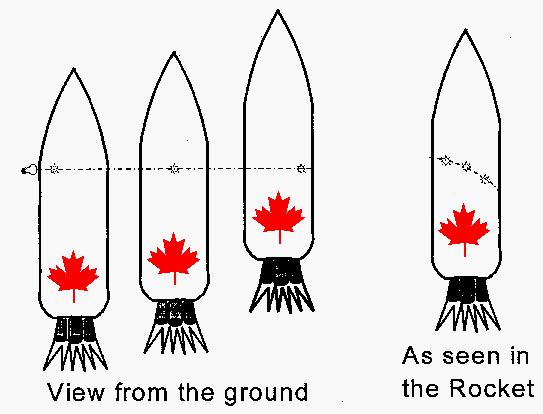
\includegraphics[width=8cm, height=5cm]{relgen3.jpg}
  \caption{Geodesic can be curved by acceleration}
  \label{fig:rocket}
 \end{figure}

 빛은 Geodesic이라는 고유한 측지선을 따라 운동한다고 하였는데 빛이 휘었다는 것은 즉, Geo-desic 자체가 휘어있다고 생각할 수 있다. 좀 더 쉽게 말하면, 빛은 직진하는데 그 '직진'이라는 것이 휜 것으로 보인다면 공간, 즉, 시공간
 자체가 휘어있다고 볼 수 있는 것이다. 이때, 관성력은 중력과 같다고 하였으므로 중력 역시 시공간을 휘게 할 것이고 이것이 대략적인 일반상대론의 postulate이다. 너무 말로만 하는 것은 필자도 힘들고 여러분들도 지루할 것이므로 
 이제 그만 우리의 목표를 말하고 Introduction을 마치도록 하자. 우리의 목표는 바로 다음 방정식을 유도(Derive)하는 것이다.
 
 \begin{equation}
  G_{ab} + \Lambda g_{ab} = 8\pi G T_{ab}
 \end{equation}

 간략히 설명하고 넘어가자면 좌변의 $G_{ab}$는 Geometric을 대표하는 Tensor로 Einstein Tensor로 불리며 Contracted Bianchi identity를 만족시키기 위하여 Ricci tensor와 Ricci scalar를 
 적절히 조합한 것이다. 우변의 $T_{ab}$는 Energy-Momentum tensor로 Matter를 대표한다. (물질의 에너지나 운동량이 시공간을 휘게한다 생각하면 쉽다.) 마지막으로 $\Lambda$는 단순히 Uniqueness문제에서 
 튀어나온것이므로 일종의 Generate scalar라고 생각하면 된다. (이것이 엄청난 존재가 될 것이라는건 함정...)
%------------------------------------------------

\section{Postulate \& Mathematical Preliminaries}
\subsection{Equivalence Principle}


\HS 전자기학에서 우리는 scalar potential과 charge density간의 관계에 대하여 다음과 같은 방정식을 배웠다. 그 유명한 Gauss' Law이다.

\begin{equation*}
 \nabla^2 \Phi = -4\pi\rho (r)
\end{equation*}

그리고 이것은 당연하게도 중력에도 적용된다. 그리고나서 풀어보면 다음과 같은 결과를 얻을 수 있다.


\begin{gather}
   \nabla^2 \Phi = 4\pi G \rho \\
   \Phi (r,t) = -G \int d^3 r' \frac{\rho (r',t)}{|r-r'|}
\end{gather}

그리고 우리는 여기서 이 결과가 특수상대론에 위배된다는 것을 바로 알 수 있다.

\begin{enumerate}
 \item Lorentz transform : 식 (2.1)에서 밀도와 공간의 이계 미분과의 상관관계를 알 수 있지만, 시간의 미분 항이 없다.
 \item Simultaneous in differential inertial frames : 세기는 공간상의 거리에 구애받지만, 전달시간은 항상 0이다.
\end{enumerate}

고로 뉴턴의 중력이론은 특수상대론과 incompatible함을 알 수 있다. 따라서 우리는 다른 이론, 즉, General Relativity가 필요함을 자명하게 느낄 수 있다.
이를 위해 등가원리라 불리는 두 가지 전제를 해보자.

\begin{enumerate}
 \item Weak Equivalence Principle : (Uniform한) 중력장은 균일한 가속과 구분할 수 없다.
 \item Local inertial Frame : 일반상대론에서의 local frame은 Minkowski space-time에서의 관성계와 같다.
\end{enumerate}

즉, 일반상대론은 Topology에 의해 기술되는 Global한 이론이 아니라 Differential Geometry의 가용범위인 Local한 이론임을 알 수 있다. \hspace{0.1cm} 그럼 이제 미분기하학을 
알아보도록 하자.
%------------------------------------------------

\subsection{Manifold \& Tensors}

\HS Manifold란 Continuously parametrize 할 수 있는 모든 집합을 일컫는다. 물리에서는 특별히 Differentiable manifolds에 관심이 많은데 이는 manifold의 모든
 open cover들에 대하여 동일 dimension을 가지는 Euclidean space의 open set으로의 injective map이 존재하고, 그 map이 smooth 할 때의 manifold이다.\footnotemark
\footnotetext{자세한 정의는 Harvey Reall을 참조하길 바란다.}
이때, smooth한 injective map을 chart라 부르고 (보통 $\phi_{\alpha}$로 나타낸다.) chart들의 집합을 atlas라고 부른다.

\VS

\HS 즉, 쉽게 설명하자면 모든 Differentiable Manifold에는 그것과 동일 차원의 Euclidean space가 reference frame으로 따라붙고 이때, Manifold 로부터 실수공간으로의 
미분가능한 함수가 chart이다. 예를 들어, 1차원 구 공간 (=원) $S^1$은 모든 점마다 $\cos \theta, \sin \theta$ 같은 미분가능한 chart가 $\theta$라는 $\mathbb{R}$ 공간안의 변수들과의 연결고리가 된다.
이제 좀 더 재미있는 짓을 하기 위하여 Manifold에서 $\mathbb{R}$로 가는 함수 $f$를 생각해보자. 우리는 미분가능한 함수에 관심이 많으니 이 $f$라는 함수도 미분가능하게 만들면 될 것이다.
그러나 문제는 이것의 domain이 Manifold($\mathcal{M}$)라는데에 있다. 보통 Calculus는 Euclidean space에서 정의되기 때문에 Manifold에서 정의된 함수의 미분가능성은 직접적으로는 보일 수 없다.
다만, 이것이 Differentiable Manifold라면 smooth한 함수인 chart를 이용하여 Euclidean space에서 $\mathbb{R}$로 가는 함수를 다음과 같이 만들 수 있다.
\begin{equation*}
 F \equiv f \circ \phi^{-1} :\hspace{0.1cm} \mathcal{U} \rightarrow \mathbb{R}
\end{equation*}
이때, $\phi:\hspace{0.1cm} \mathcal{M} \rightarrow \mathbb{R}^n$ 이며 $\mathcal{U} \subset \mathbb{R}^n$ 이다. 따라서 우리는 이제 $F$의 미분가능성을 판별할 수 있고, 
이로 하여금 $f$의 미분가능성을 간접적으로 확인할 수 있다. 여기서 자연스레 드는 의문. 도대체 왜 이 짓을 하고 있냐? 바쁜 사람들을 위한 상대론이라면서 뭔 정의를 다 따지고 있냐?

그러나 눈치 빠른 사람이라면 알아챘겠지만, 여기서의 $f$는 모든 Manifold 상의 점으로부터 숫자를 Generate하므로 일반상대론에서 쓰이는 용어로는 Scalar Field라고 한다.
그리고 당연하게도 앞으로 할 Vector, Covector 같은 개념을 다루려면 Scalar Field의 개념은 탄탄하게 다져놓아야 한다.\footnotemark
\footnotetext{만약, 이것을 확실히 다져놓고 싶다면 Sage manifolds를 검색하여 다운받은 후 구동하여 Manifold 상에서 Klein-Gordon Lagrangian이라도 만들어 보길 바란다.
 진정으로 분노가 솟아오르면서 자연스레 이해될 것이다.}
 
 \VS
 
 \HS 자, 그러면 Scalar는 해결되었으니 이제 Vector를 보자. 그런데 Manifold위에서 Vector를 어떻게 정의해야 할까? Manifold 표면이 곡면이면 Vector도 곡선이어야 할까?
 이러한 문제제기를 회피하기 위하여 우리는 Local하게 접근해야할 필요가 있다. (애초에 General Relativity도 Local Theory이다.)
 즉, Manifold 상의 모든 각각의 점들에 대하여
 Tangent Space 혹은 Tangent Plane을 구축하는 것이다! 이것을 구축하고 나면 그 안의 모든 원소를 Vector라고 보면 되니 되게 정의하기 쉬워졌다.\footnotemark
 \footnotetext{만약 이것이 잘 이해가 되지 않는다면 구글에 Tangent Plane을 검색해보기를 권한다.}
 이때, Tangent Space의 기호는   $T_{p} (\mathcal{M})$ 으로 쓴다. 그럼 이제 보다 벡터를 더 구체적으로 정의하기 위하여 Manifold위에 smooth curve인 $\lambda$를 정의하자.
 자명한 이야기지만 curve는 하나의 변수로 parametrize 되므로 $\lambda$는$I\subset\mathbb{R}$인 $I$에 대하여 $I \rightarrow \mathcal{M}$ 인 함수이다. 그렇다면, 우리는
 직감적으로 $ f \circ \lambda$가 $I \rightarrow \mathbb{R}$ 인 smooth한 1차원 함수이고, 따라서 흔히 알려진 미분방법으로 미분할 수 있다는 것을 알 수 있다.
 이때, $\lambda$를 parametrize하는 변수를 $t$라 하고, $\lambda (a) = p$ 라고 해보자. 그렇다면 우리는 Tangent Vector를 다음과 같이 정의할 수 있다.
 
 \begin{equation}
  X_p (f) = \frac{d}{dt} [f(\lambda (t))]_{t=a}
 \end{equation}

 이때, Tangent Vector $X_p$는 $L(\mathcal{M}, \mathbb{R})$의 원소이고,  Manifold 상의 한 점 p에 대하여 모든 Tangent Vector들을 모은 공간이 $T_p (\mathcal{M})$이 된다.
 여기까지는 전혀 상대론의 기미가 보이지 않아 지루할 수 있겠으나, 바로 지금 무언가 재미있는 것을 볼 수 있다.
 
\HS $f\circ\lambda = (f\circ\phi^{-1})\circ (\phi\circ\lambda)=F\circ(\phi\circ\lambda)$ 임을 이용하여 다시 한번 $X_p (f)$를 전개하면 다음을 얻을 수 있다.

\begin{equation}
 \label{eq:tan}
 X_p (f) = \frac{d}{dt}[F(\phi(\lambda (t)))]_{t=a} = \left( \frac{\partial F(x)}{\partial x^{\mu}} \right)_{\phi(p)} \left(\frac{dx^{\mu}(t)}{dt}\right)_{t=a}
\end{equation}

그렇게 어려운 식은 아니지만 처음이라 적응이 잘 안될테니 한번 살펴보자. 일단 상대론에서는 Einstein summation convention 이라는 것을 사용한다. 말은 거창하지만 내용은 
그냥 $\sum$ 기호 쓰기 귀찮으니 생략하자! 이다. 따라서 index ($\mu, \nu$ 같은) 들이 붙어있는 것에는 $\sum$가 생략되어 있다고 생각하면 된다.\footnotemark
\footnotetext{자세한 것은 역시 구글을 참조하자.}
다음으로 등식자체를 보면, 아마 마지막 등식으로 넘어가는 징검다리를 찾기가 힘들 것이다. 이는 chart가 알게 모르게 들어가 있어서 그런 것인데, 한번 짚고 넘어가자.
앞에서 chart를 설명할 때 Manifold에서 Euclidean space로 가는 smooth한 함수라고 정의하였는데 이를 생각해보면 Manifold상의 한 점 p에 대하여 $\phi(p)$는 Euclidean space의
한 점이다. 이는 마치 3차원 구의 표면상의 한 점을 나타내고자 할 때, $(x,y,z)$라는 3차원 Euclidean space의 점이 필요한 것과 같다. 그리고 이를 보통 $x^{\mu}$로 나타낸다.
즉, $\phi = \{ x^1 , x^2 , \cdots \} = \{ x^{\mu} \}$ 이므로 간단히 chain rule을 사용하면 식 \ref{eq:tan} 와 같은 결과를 얻을 수 있다. 그럼 이제 한번 더 나아가보자.

\begin{equation}
 X_p (f) = \BKS{ \PD{}{x^{\mu}} }_p (f) \BKS{\OD{x^{\mu}(t)}{t}}_{t=a} = \BKS{\OD{x^{\mu}(t)}{t}}_{t=a} \Basis (f)
\end{equation}

이때, 양 변에서 input에 지나지 않는 $f$는 지워버리면 단순히 다음과 같이 된다.

\begin{equation}
 \label{eq:basis}
 X_p = \BKS{\OD{x^{\mu}(t)}{t}}_{t=a} \Basis
\end{equation}

\HS 그럼 이제 앞에서 말했던 $X_p \in T_p (\Manifold)$를 사용하면 우리는 $X_p = X^{\mu} e_{\mu}$ 로 나타낼 수 있다. 이때, $X^{\mu}$는 벡터 $X_p$의 component이고 $e_{\mu}$는
$\Tangent$의 Basis이다. 이 정의를 이용하면 앞의 식 \ref{eq:basis}에서 $\Basis$ 가 Basis 이며 $X^{\mu} = \BKS{\OD{x^{\mu}}{t}}_{t=a}$임을 알 수 있다. \footnotemark
\footnotetext{좀 더 일반적으로 말하자면, $\Basis$ 는 \emph{Coordinate Basis} 라고 부르며 일반적으로는 $e_{\mu}$ 를 Basis로 둔다.}

\VS

\paragraph{$-$Contravariant}

앞에서 $\Tangent$ 와 basis 얘기를 했는데 당연하게도 basis는 unique할 이유가 없다. 따라서 우리는 basis를 다양하게 바꿔볼 수 있다. 그러나 주의해야 할 것은
basis를 바꾸면 자연스럽게 component도 바뀐다는 것이다. 여기서는 앞에서 다뤘던 순수한 vector에 대해서 basis 변환을 볼 것이다. 여기서 basis를 변환한다는 것은 곧
chart를 바꾸는 것과 같기때문에 한 점 $p$에 대하여 두 가지 chart ($\phi,\hspace{0.1cm} \phi'$)를 가정해보자. 그렇다면 우리는 벡터의 정의를 이용하기 위하여 다음과 같이 설정할 수 있다.

\begin{equation*}
 f\circ\phi^{-1} = (f\circ\phi'^{-1})\circ(\phi'\circ\phi^{-1}) \equiv F'\BKS{x'^{\nu} (x)}\footnotemark
\end{equation*}

\footnotetext{부가 설명을 하자면, $F'$d은 앞에서의 정의와 같고 $\phi'=\{x'^{\nu}\}$ 이고 마지막으로 $\phi^{-1}$는 input으로 $\phi$를 받아야 하므로 식의 형태가 이렇게 된다.}
그럼 이제 식을 전개해보자.

\begin{equation}
  \begin{split}
    \Basis (f) & = \BKS{\PD{}{x^{\mu}} (f\circ\phi^{-1})}_{\phi(p)} = \BKS{\PD{}{x^{\mu}} \left[ (f\circ\phi'^{-1})\circ(\phi'\circ\phi^{-1}) \right]}_{\phi(p)} \\
    & \equiv \PD{}{x^{\mu}} \BKS{F'(x'^{\nu}(x))}_{\phi(p)} = \BKS{\PD{x'^{\nu}(x)}{x^{\mu}}}_{\phi(p)}\BKS{\PD{F'(x')}{x'^{\nu}}}_{\phi'(p)} \\
    & = \BKS{\PD{x'^{\nu}}{x^{\mu}}}_{\phi(p)}\BKS{\PD{}{x'^{\nu}}}_p (f)
  \end{split}
\end{equation}

즉, 앞에서 했던 방식처럼 $f$를 제외한 함수부분만 보면 결국 다음이 된다는 것을 알 수 있다.

\begin{equation}
 \therefore \Basis = \BKS{\PD{x'^{\nu}}{x^{\mu}}}_{\phi(p)}\BKS{\PD{}{x'^{\nu}}}_p
\end{equation}

그럼 마지막으로 이를 이용하여 벡터의 기저변환을 볼 수 있다.
\begin{gather}
 X = X^{\mu} \Basis = X^{\mu} \BKS{\PD{x'^{\nu}}{x^{\mu}}}_{\phi(p)} \BKS{\PD{}{x'^{\nu}}}_p \equiv X'^{\nu} \BKS{\PD{}{x'^{\nu}}}_p \\
 \therefore X'^{\nu} = X^{\mu} \BKS{\PD{x'^{\nu}}{x^{\mu}}}_{\phi(p)}
\end{gather}

이런 변환을 갖는 벡터를 \emph{Contravariant Vector} 라고 한다.

\pagebreak

\paragraph{$-$Covector} 지금까지 열심히 Manifold 위에서 Vector를 정의하는 법을 배웠다. Vector의 정의는 Manifold상의 curve인 $\lambda$를 Scalar field에 넣어 숫자로 만든 후 한 점 p에서 
그것을 curve의 parameter에 대하여 미분한 것이다. 즉, 간단히 말하자면 Vector는 Scalar field를 미분하여 실수로 보내버리는 Linear map이다. 물론 Divergence같은 scalar quantity도 중요하지만
우리는 또한 Vector량인 Gradient가 중요함을 알고 있다. 이것을 Manifold상에서 정의하기 위하여 미분기하학의 1-form 개념을 이용해보자. 1-form은 기본적으로 어떤 Vector space에 대하여
Vector space를 실수로 보내버리는 Linear map이기 때문에 우리는 그러한 공간을 정의할 필요가 있다. 우리가 정의한 Vector Space는 단 하나, $\Tangent$ 뿐이므로 그것을 Linear하게 mapping하는
공간을 정의할 수 있는데 이 공간을 \emph{Tangent Space의 Dual space} 혹은 \emph{Cotangent Space}라 부르며 기호로는 $\Cotangent$ 라고 쓴다. 
그리고 이 공간에 속하는 원소들을 p에서의 \emph{1-form} 혹은 \emph{Covector}라고 부르며 보통 기호로는 $\eta$라고 쓴다. 그리고 앞에서 벡터를 Component와 Basis로 나누었던 것 처럼 
Covector 역시 나눌 수 있다.

\begin{equation*}
 \eta = \eta_{\mu} f^{\mu} \HS where \hspace{0.2cm} f^{\mu} (e_{\nu}) = \delta^{\mu}_{\nu}
\end{equation*}

그리고 Covector 의 성질은 다음과 같다.

\begin{gather*}
 \eta(e_{\nu}) = \eta_{\mu} f^{\mu}(e_{\nu}) = \eta_{\mu} \delta^{\mu}_{\nu} = \eta_{\nu} \\
 \eta(X) = \eta(X^{\mu} e_{\mu}) = X^{\mu} \eta (e_{\mu}) = X^{\mu} \eta_{\mu}
\end{gather*}

앞의 벡터에서 특히 $\Basis$ 를 Coordinate Basis라고 불렀는데 (각주 9번 참조) 마찬가지로 Covector에도 특수한 기저가 존재한다. 일단 다음을 보자.

\begin{equation}
\label{eq:CC}
 (df)_p (X) \equiv X(f)
\end{equation}

여기에서 $f=x^{\mu}$ 가 바로 Covector의 Coordinate Basis이다. 이것의 성질을 한번 알아보자.

\begin{gather}
\label{eq:dual}
 (dx^{\mu})_p \BKS{\PD{}{x^{\nu}}_p} = \BKS{\PD{x^{\mu}}{x^{\nu}}}_{\phi(p)} = \delta^{\mu}_{\nu} \\
 \left[ (dx^{\mu})_p \right] _{\nu} = (dx^{\mu})_p \BKS{\PD{}{x^{\nu}}}_p = \BKS{ \PD{}{x^{\nu}}_p } \BKS{x^{\mu}} = \BKS{\PD{x^{\mu}}{x'^{\nu}}}_{\phi'(p)} \BKS{\PD{x'^{\nu}}{x^{\nu}}}_{\phi(p)}
 = \BKS{\PD{x^{\mu}}{x'^{\nu}}}_{\phi'(p)} \left[ (dx'^{\nu})_p \right]_{\nu}
 \label{eq:covector}
\end{gather}

\pagebreak

\HS 식 \ref{eq:dual} 에서 우리는 Covector의 Coordinate Basis가 Vector의 Coordinate Basis와 Dual관계임을 알 수 있다. 다음으로 식 \ref{eq:covector}을 보면 2번째 식에서 3번째 식으로 넘어갈 때는
식 \ref{eq:CC} 에서의 정의를 이용하였고 나머지는 그저 계산으로 이루어져있다. 이것을 이용하면 Covector의 Basis transform에 의한 Component difference를 알 수 있다.

\begin{gather}
 \therefore (dx^{\mu})_p = \BKS{\PD{x^{\mu}}{x'^{\nu}}}_{\phi'(p)} (dx'^{\nu})_p \\
 \therefore \eta'_{\mu} = \BKS{\PD{x^{\nu}}{x'^{\mu}}}_{\phi'(p)} \eta_{\nu} 
 \label{eq:covariant}
\end{gather}

식 \ref{eq:covariant}를 만족하는 quantity를 \emph{Covariant Vector} 라고 한다.

\paragraph{$-$Tensors}

지금까지 뭔가 엄청난걸 한 것 같지만 사실 Vector와 Covector (=Dual Vector) 두 가지 밖에 하지 않았다. 이것들로 Gradient나 Divergence같은 기본적인 미적분학은 다룰 수 있지만
일반상대론에서 가장 중요한 '곡률' (Curvature) 이란 개념을 다루지 못한다. 이것을 다루기 위해서는 Tensor라는 괴상한 존재가 필요하다. 
텐서는 지금까지 해왔던 Vector나 Covector 개념들의 상위호환 (그것도 엄청난!) 이라고 생각하면 된다. 이게 엄청난 것이 때에 따라 Vector도 될 수 있고 Covector 역시 될 수 있으며 심지어
원래는 서로서로 보내버리기에 급급했던 Vector나 Covector들을 참교육 시켜서 두 개 이상의 Vector나 Covector들을 사이좋게 1차원 실수로 만들어 버릴 수 있다. \sout{마인부우?!} \Hs 아무튼 텐서의 정의는 다음과 같다.

\vspace{0.4cm}

\begin{defn}
 A Tensor of type $(r,s)$ at $p$ is a multi-linear map 
 \begin{equation*}
  T : \Hs \Cotangent \times \cdots \times \Cotangent \times \Tangent \times \cdots \times \Tangent \rightarrow \mathbb{R}
 \end{equation*}
 where there are $r$ factors of $\Cotangent$ and $s$ factors of $\Tangent$
\end{defn}

\VS

즉, $r$개의 Covector들과 $s$개의 Vector들을 실수로 보내버리는 Multi-linear 함수가 Tensor이다. 이때의 Tensor type을 $(r,s)$라 부르자는게 약속이다. 
그렇다면 $(0,1)$ Tensor는 무엇일까? 0개의 Covector, 1개의 Vector 즉, Vector를 실수로 보내버리므로 바로 Covector이다. 마찬가지로 $(1,0)$ Tensor는 Covector를 실수로 보내버리므로
Vector이다. 이제 대략적인 Tensor의 개념을 알았으니 중요한 것은 Tensor의 Component를 어떻게 기술할 것인지가 될 것이다. 우리는 이미 다음 사실을 알고있다.

\begin{gather*}
 X(f^{\mu}) = X^{\nu}e_{\nu}(f^{\mu}) = X^{\nu} \KD = X^{\mu} \\
 \eta(e_{\nu}) = \eta_{\mu} f^{\mu}(e_{\nu}) = \eta_{\mu} \KD = \eta_{\nu}
\end{gather*}

즉, Component를 구하는 방법은 input으로 Domain space의 Basis를 넣어주는 것이다. 고로 우리는 Tensor의 Component를 다음과 같이 정의할 수 있다.


\begin{defn}
 The components of tensor $T$ of type $(r,s)$ at $p$ is
 \begin{equation*}
  \tensor{T}{^{\mu_1}^{\mu_2}^{\cdots}^{\mu_r}_{\nu_1}_{\nu_2}_{\cdots}_{\nu_s}} = T \BKS{f^{\mu_1},f^{\mu_2},\cdots,f^{\mu_r},e_{\nu_1},e_{\nu_2},\cdots,e_{\nu_s}}
 \end{equation*}

\end{defn}

\VS

\paragraph{$-$Change of Coordinate Basis}

우린 이미 Vector와 Covector에서 Coordinate Basis를 변환할 때, Component가 어떻게 변하는지에 대하여 다뤄보았다. 그러나 매번 Chain rule에 의존하여 유도하다가는
제 명에 못 죽을 것이 분명하다. 따라서 여기서는 Matrix Form으로 변환들을 정리하면서 Tensor에서의 변환은 어떻게 될지 다뤄보고자 한다. 그 결과는 다음과 같다.

\VS

\begin{enumerate}
 \item Vector: \Hs $\begin{aligned}[t]
                     X = X^{\nu}e_{\nu} = X^{\nu} \BKS{\PD{x'^{\mu}}{x^{\nu}}}_p e'_\mu \Hs \Longrightarrow \Hs X'^{\mu} = X^{\nu}\BKS{\PD{x'^{\mu}}{x^{\mu}}}_p \equiv \tensor{A}{^\mu _\nu}X^{\nu}
                    \end{aligned}$
 \item Covector: \Hs $\begin{aligned}[t]
                       \eta = \eta_{\nu} f^{\nu} = \eta_{\nu} \BKS{\PD{x^{\nu}}{x'^{\mu}}}_p f'^{\mu} \Hs \Longrightarrow \Hs \eta'_{\mu} = \eta_{\nu} \BKS{\PD{x^{\nu}}{x'^{\mu}}}_p \equiv \tensor{\BKS{A^{-1}}}{^\nu _\mu}\eta_{\nu}
                      \end{aligned}$
 \item Tensor: \Hs $\begin{aligned}[t]
                     T(\eta,\omega,X) & = \tensor{T}{^\sigma^\tau_\lambda} \eta_\sigma \omega_{\tau} X^{\lambda}\\
                     \tensor{T}{^\sigma ^\tau _\lambda} & = T(f^\sigma, f^\tau,e_\lambda) = \tensor{\BKS{A^{-1}}}{^\sigma _\mu} \tensor{\BKS{A^{-1}}}{^\tau _\nu} \tensor{A}{^\rho _\lambda} \tensor{{T'}}{ ^\mu ^\nu _\rho} \\
                     \tensor{{T'}}{^\mu ^\nu _\rho} & = \tensor{A}{^\mu _\sigma} \tensor{A}{^\nu _\tau} \tensor{\BKS{A^{-1}}}{^\lambda _\rho} \tensor{T}{^\sigma^\tau_\lambda} 
                    \end{aligned}$


\end{enumerate}


\paragraph{$-$ Contraction}

Y대학교 물리학과 수업에는 엄청난(?) 수업이 하나 있다. 2013학년도부터 일반역학이라 시행된 그 수업은 사실 고전장론을 다루는 수업이다.\footnotemark
\footnotetext{학생들의 무궁한 항의에 의해 2016년도부터는 현대물리의 이름을 달고 있다.}
이 수업은 기본적으로 Landau 2권인 \emph{The Classical theory of the fields} 의 요약판인데 이 책의 특징은 수학적엄밀성을 버리는 대신 직관에 치중하자 이기에 
쉽지만 찜찜함이 남는 책이다. 이 책에서는 Contraction 이란 \textit{upper index와 동일한 lower index가 만나면 rank가 하나 내려가게 되는 것} 이다. 실로 찜찜하지 않을 수 없다.
여담으로 이 교수님(\sout{코드명: zero-one})은 2016년도에 이르러 일반상대론입문이라는 수업을 열게 되었고 필자는 눈물을 훔치며 낚여 나가는 물리학도생들의 참상을 목도할 수 밖에 없었다. \footnotemark 
\footnotetext{혹여 Y대학에 들어가 이 수업을 들으려 고민한다면, 당장 주저하지말고 그러한 생각을 한 자신조차 반성하라. 만약 상대론에 입문을 하고 싶은 자는 서점으로 가서 란다우 책을 구입한 뒤 그냥 읽는게 더 이득이다.}

\pagebreak

\HS 자 그렇다면 본격적으로 Contraction 이라는 것을 보다 엄밀하게 다뤄볼텐데 이해를 쉽게 하기 위하여 $(3,2)$ Tensor를 예로 들어 설명하겠다. 그러나 일반적인 $(3,2)$ 가 아니라 하나의 Covector basis 와 하나의 Vector basis가 같은, 다음과 같은 경우를 고려해보자.

\begin{equation*}
 T(f^{\mu},\omega,\nu,e_{\mu},X)
\end{equation*}

보기엔 별 것 아닌 것 같지만 $f$ 와 $e$ 를 다른 Basis로 change해보면 굉장히 재미있는 성질이 나타난다.

\begin{align}
\begin{split}
 T(f'^{\mu},\omega,\nu,e'_{\mu},X) &= T(\CT f^{\nu}\Com \omega\Com \eta\Com \CTI[\rho][\mu]e_\rho\Com X)\Hs = \CT \CTI[\rho][\mu] T(f^\nu, \omega, \eta, e_\mu, X) \\
 & = \KD[\rho][\nu] T(f^\nu, \omega,\eta,e_\rho,X)\Hs = \Hs T(f^\mu,\omega,\eta,e_\mu,X)
\end{split}
\end{align}

\VS

고로 $f$와 $e$는 Basis 변환에서 자유롭다는 것을 확인할 수 있다. 이는 바꿔말하면 이 텐서는 $f$와 $e$에 대하여 Independent하다는 것이고 즉, (3,2) Tensor가 아니라
(2,1) Tensor와 같은 역할을 함을 알 수 있다. 이것을 Abstract notation\footnotemark 으로 나타내면 다음과 같다.
\footnotetext{이것에 대하여 굳이 설명하긴 \sout{귀찮} 힘드므로 Harvey reall의 part3. General Relativity 강의노트 2.6을 참조하라. 구글에 검색하면 바로 나온다.}
\begin{equation}
 \tensor{T}{^d ^a ^b _d _c} = \tensor{S}{^a ^b _c }
\end{equation}

간단히 기술적으로만 말하면 위 아래에 같은 index가 있으면 어차피 그것에 대한 의존성은 사라지므로 Tensor type이 바뀌는 것과 같다.

\paragraph{$-$ Supplement}

\begin{itemize}
 \item $T_{(ab)} = \frac{1}{2} \BKS{T_{ab} + T_{ba}}\Com\Hs T_{[ab]} = \frac{1}{2}\BKS{T_{ab} - T_{ba}  }$
 \item $\tensor{T}{^a^b_c} \neq \tensor{T}{_c ^a ^b}$ : 앞의 것은 $\Cotangent\times\Cotangent\times\Tangent \rightarrow \mathbb{R}$ 인데 뒤의 것은 
 
 $\Tangent\times\Cotangent\times\Cotangent\rightarrow\mathbb{R}$ 이므로 서로 다르다. 따라서 기본적으로 앞의 것을 쓰기로 밀약을 해놓는다.
\end{itemize}

\pagebreak

\paragraph{$-$The Commutator} 이 토픽을 시작하기 전에 먼저 개념 하나를 제시하고자 한다. 지금까지 앞에서 한 모든 것들은 결국 Manifold 상의 한 점 $p$에서 벌어진 일들이다.
하지만 우린 결코 한 점만 다룰 것이 아니므로 개념을 좀 확장해보자. 거의 초반에 우리는 Scalar Field를 공부하였다. 그렇다면 Vector나 Covector 심지어 Tensor도 모든 점에서 정의되게끔
Field로 정의한다면 아주 편하게 Manifold 전체를 아우를 수 있을 것이다. 따라서 이제부터 쓰는 Tensor들은 별다른 언급이 없으면 모두 Field라 봐도 무방하다. 그럼 시작해보자.

\HS 이번에는 두 개 이상의 Vector field들을 합성하여 새로운 Vector Field를 만드는 것을 한 번 해보자. 먼저 당연하게 단순한 Composition field인 $X(Y(f))$를 생각해 볼 수 있다.
그러나 조금만 보면 이것이 Vector Field가 아니라는 것을 확인할 수 있다.

\begin{equation}
\label{eq:nonvec}
 X(Y(fg))\Hs =\Hs X(fY(g)+gY(f)) = fX(Y(g)) + gX(Y(f)) + X(f)Y(g) + X(g)Y(f)
\end{equation}

보면 알겠지만, 혹은 모를 수도 있겠지만 기본적으로 Field들은 Leibniz Rule\footnotemark 을 만족하여야 한다. 그러나 보다시피 $X(Y(f))$는 만족하지 않는다. 
\footnotetext{$X(fg) = X(f)g + fX(g)$}
이것을 만족하게 하려면 식 \ref{eq:nonvec}에서 뒤의 두 항이 사라져야함을 알 수 있는데, 뒤의 두 항은 Symmetric하므로 쉽게 없앨 수 있다.

\begin{equation}
 \RCommutator{fg}\Hs=\Hs f\BKS{\RCommutator{g}} + g\BKS{\RCommutator{f}}
\end{equation}

따라서 $\RCommutator{f}$는 Vector Field임을 알 수 있고, 이를 Commutator라 부르며 다음과 같이 쓴다.

\begin{equation}
 \Commutator(f) = \RCommutator{f}
\end{equation}

이것을 Coordinate Basis를 사용하여 index를 넣어 표현하면 다음과 같다.

\begin{align}
 \begin{split}
  \Commutator(f) & = X\BKS{Y^\nu \PD{F}{x^\nu}} - Y\BKS{x^\mu \PD{F}{x^\mu}} = X^\mu \Basisnp \BKS{Y^{\nu}\PD{F}{x^\nu}}-Y^\nu \BKS{\PD{}{y^\nu}}\BKS{X^\mu \PD{F}{x^\mu}} \\
                 & = X^\mu\BKS{\PD{Y^\nu}{x^\mu}}\BKS{\PD{F}{x^\mu}} - Y^\nu\BKS{\PD{X^\mu}{x^\nu}}\BKS{\PD{F}{x^\mu}} \\
                 & = \ECommutator \BKS{\PD{F}{x^\mu}} \equiv \Commutator^\mu \BKS{\PD{F}{x^\mu}}
 \end{split}
\end{align}

\begin{equation}
 \therefore \Commutator^\mu = \ECommutator
\end{equation}

%----------------------------------------------------------------------------------------
%	PROBLEM 2
%----------------------------------------------------------------------------------------



%------------------------------------------------



%------------------------------------------------



%----------------------------------------------------------------------------------------

\end{document}